%
% This is a borrowed LaTeX template file for lecture notes for CS267,
% Applications of Parallel Computing, UCBerkeley EECS Department.
% Now being used for CMU's 10725 Fall 2012 Optimization course
% taught by Geoff Gordon and Ryan Tibshirani.  When preparing 
% LaTeX notes for this class, please use this template.
%
% To familiarize yourself with this template, the body contains
% some examples of its use.  Look them over.  Then you can
% run LaTeX on this file.  After you have LaTeXed this file then
% you can look over the result either by printing it out with
% dvips or using xdvi. "pdflatex template.tex" should also work.
%

\documentclass[twoside]{article}
\setlength{\oddsidemargin}{0.25 in}
\setlength{\evensidemargin}{-0.25 in}
\setlength{\topmargin}{-0.6 in}
\setlength{\textwidth}{6.5 in}
\setlength{\textheight}{8.5 in}
\setlength{\headsep}{0.75 in}
\setlength{\parindent}{0 in}
\setlength{\parskip}{0.1 in}

%
% ADD PACKAGES here:
%

\usepackage{amsmath,amsfonts,graphicx}

%
% The following commands set up the lecnum (lecture number)
% counter and make various numbering schemes work relative
% to the lecture number.
%
\newcounter{lecnum}
\renewcommand{\thepage}{\thelecnum-\arabic{page}}
\renewcommand{\thesection}{\thelecnum.\arabic{section}}
\renewcommand{\theequation}{\thelecnum.\arabic{equation}}
\renewcommand{\thefigure}{\thelecnum.\arabic{figure}}
\renewcommand{\thetable}{\thelecnum.\arabic{table}}

%
% The following macro is used to generate the header.
%
\newcommand{\lecture}[4]{
   \pagestyle{myheadings}
   \thispagestyle{plain}
   \newpage
   \setcounter{lecnum}{#1}
   \setcounter{page}{1}
   \noindent
   \begin{center}
   \framebox{
      \vbox{\vspace{2mm}
    \hbox to 6.28in { {\bf EE302 - Feedback Systems
	\hfill Spring 2019} }
       \vspace{4mm}
       \hbox to 6.28in { {\Large \hfill Lecture #1 \hfill} }
       \vspace{2mm}
       \hbox to 6.28in { {\it Lecturer: #2 \hfill } }
      \vspace{2mm}}
   }
   \end{center}
   \markboth{Lecture #1}{Lecture #1}

   \vspace*{4mm}
}
%
% Convention for citations is authors' initials followed by the year.
% For example, to cite a paper by Leighton and Maggs you would type
% \cite{LM89}, and to cite a paper by Strassen you would type \cite{S69}.
% (To avoid bibliography problems, for now we redefine the \cite command.)
% Also commands that create a suitable format for the reference list.
\renewcommand{\cite}[1]{[#1]}
\def\beginrefs{\begin{list}%
        {[\arabic{equation}]}{\usecounter{equation}
         \setlength{\leftmargin}{2.0truecm}\setlength{\labelsep}{0.4truecm}%
         \setlength{\labelwidth}{1.6truecm}}}
\def\endrefs{\end{list}}
\def\bibentry#1{\item[\hbox{[#1]}]}

%Use this command for a figure; it puts a figure in wherever you want it.
%usage: \fig{NUMBER}{SPACE-IN-INCHES}{CAPTION}
\newcommand{\fig}[3]{
			\vspace{#2}
			\begin{center}
			Figure \thelecnum.#1:~#3
			\end{center}
	}
% Use these for theorems, lemmas, proofs, etc.
\newtheorem{theorem}{Theorem}[lecnum]
\newtheorem{lemma}[theorem]{Lemma}
\newtheorem{proposition}[theorem]{Proposition}
\newtheorem{claim}[theorem]{Claim}
\newtheorem{corollary}[theorem]{Corollary}
\newtheorem{definition}[theorem]{Definition}
\newenvironment{proof}{{\bf Proof:}}{\hfill\rule{2mm}{2mm}}

% **** IF YOU WANT TO DEFINE ADDITIONAL MACROS FOR YOURSELF, PUT THEM HERE:

\begin{document}

% Lecture Details
\lecture{10}{Asst. Prof. M. Mert Ankarali}

\par 

\section{PID Control Policy}

  \begin{minipage}[h]{1\linewidth}
    \begin{center}
      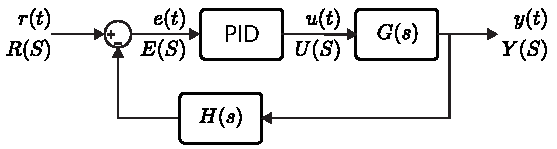
\includegraphics[width=0.6\textwidth]{PID}
    \end{center}
  \end{minipage}

A PID controller has the following forms in time and Laplace domain
%  
  \begin{align*}
  u(t) &= K_P e(t) + K_D \frac{d}{dt} e(t) + K_I \int_{0}^{t} e(t) dt
    \\
   U(s) &= \left[ K_P + K_D s + K_I \frac{1}{s} \right] E(s)
  \end{align*}
  
In this lecture we will analyze the the effects of PID coefficients on 
the transient and steady-state performance on a $2^{nd}$ order plant.
%

\subsection{Proportional (P) Controller}

Let's assume that $H(s) = 1$ and $G(s)$ is a second order
transfer function in general form 
%
  \begin{align*}
  G(s) = \frac{\omega_n^2}{s^2 + 2 \zeta \omega_n + \omega_n^2}
  \end{align*}
%
SInce $C(s) = K_P$, let's first analyze the steady-state error performance
%
\begin{align*}
  &G_{OL}(s) = \frac{K_P \omega_n^2}{s^2 + 2 \zeta \omega_n + \omega_n^2}
\\
 Type \ 0 \quad K_p = K_P
\end{align*}
% 
Thus steady-state error for unit-step and unit-ramp inputs can be find
as
\begin{itemize}
\item Unit step: $e_{ss} = \frac{1}{1 + K_P}$, i.e. $K_p \nearrow \
  \Rightarrow \ e_{ss} \searrow$  
\\ Unit ramp: $e_{ss} = \infty$
\end{itemize}
%
To sum up, higher $K_P$ provides better steady-state performance.
Now let's analyze transient performance.
%
%
  \begin{align*}
  T(s) &= \frac{Y(s)}{R(s)} = \frac{K_P \omega_n^2}{s^2 + 2 \zeta
    \omega_n  + (1 + K_P) \omega_n^2}
\\
 \bar{\omega}_n &= \sqrt{1 + K_P} \omega_n
\\
 \bar{\zeta} &= \zeta \frac{1}{ \sqrt{ 1 + K_P} } 
  \end{align*}
%
We can see that
%
  \begin{align*}
    K_p \nearrow \ &\Rightarrow \ \omega_n \nearrow \\
   K_p \nearrow \ &\Rightarrow \ \zeta \searrow  
  \end{align*}
%
If the plant is an over-damped system (i.e. $\zeta > 1$), them increasing
$\omega_n$ and decreasing $\zeta$ should has a positive net 
effect on the closed-loop performance. 

On the other hand if the plant is an under-damped system, 
we can observe the following relations 
%
\begin{align*}
\bar{\omega}_d &= \bar{\omega}_n \sqrt{1 - \bar{\zeta}^2} = \omega_n
  \sqrt{1 + K_P}  \sqrt{1 - \frac{\zeta^2}{ 1 + K_P } } 
  = \omega_n \sqrt{ 1 + K_P -\zeta^2 } 
\\
\bar{\zeta} \bar{\omega}_n &= \frac{\zeta}{ \sqrt{ 1 + K_P } }
                             \omega_n \sqrt{1 + K_P} = \zeta \omega_n
\end{align*}
%
We can see that
%
  \begin{align*}
    K_p \nearrow \ &\Rightarrow \ \omega_d \nearrow \\
   K_p \nearrow \ &\Rightarrow \ \zeta \omega_n \mathrm{=}
  \end{align*}
%
In other words real part of the complex conjugate poles
are unchanged, yet imaginary part deviates from the real 
axis. From previous lectures we kow that in this scenario
%
  \begin{align*}
    K_p \nearrow \ &\Rightarrow \ M_p \nearrow 
  \end{align*}
%
In conclusion, If the plant is an under-damped system (i.e. $\zeta <
1$), them increasing the P gains has an negative effect on 
the closed-loop performance (transient). 

\textbf{Example 1:} Let $G(s) = \frac{1}{(s+0.5)(s+5)}$ (and over-damp
plant), then compute the unit-step steady state error for $K_p = 2$ and $K_P = 5$.
%
\begin{align*}
  e_{2} &= \frac{1}{1 + 2 / 2.5} \approx 0.55 \ , (\%55) 
\\
  e_{5} &= \frac{1}{1 + 5 / 2.5} \approx 0.33 \ , (\%33) 
\end{align*}
%
Obviously, stead-state performance is better with $K_p = 5$
compared to $K_p = 1$. Now compute the closed-loop poles
for $K_p = 1$ and $K_P = 5$, and estimate associated 
settling times ($\%2$).
%
\begin{align*}
  T_2(s) = \frac{2}{s^2 + 5.5 s + 4.5} &\quad \rightarrow \
  p^{(2)}_{1} = -1 \ ,  p^{(2)}_{2} = -4.5  \quad t^{(2)}_s \approx 4
  s 
\\
  T_5(s) = \frac{5}{s^2 + 5.5 s + 7.5} &\quad \rightarrow \
  p^{(2)}_{1} = -2.5 \ ,  p^{(2)}_{2} = -3  \quad t^{(2)}_s \approx
                                         1.6 s 
\end{align*}
%
We can see that $K_P = 5$ provides a better transient performance
compared to $K_P = 2$. Now let's draw step-responses and
verify these observations

\vspace{12 pt}

  \begin{minipage}[h]{1\linewidth}
    \begin{center}
      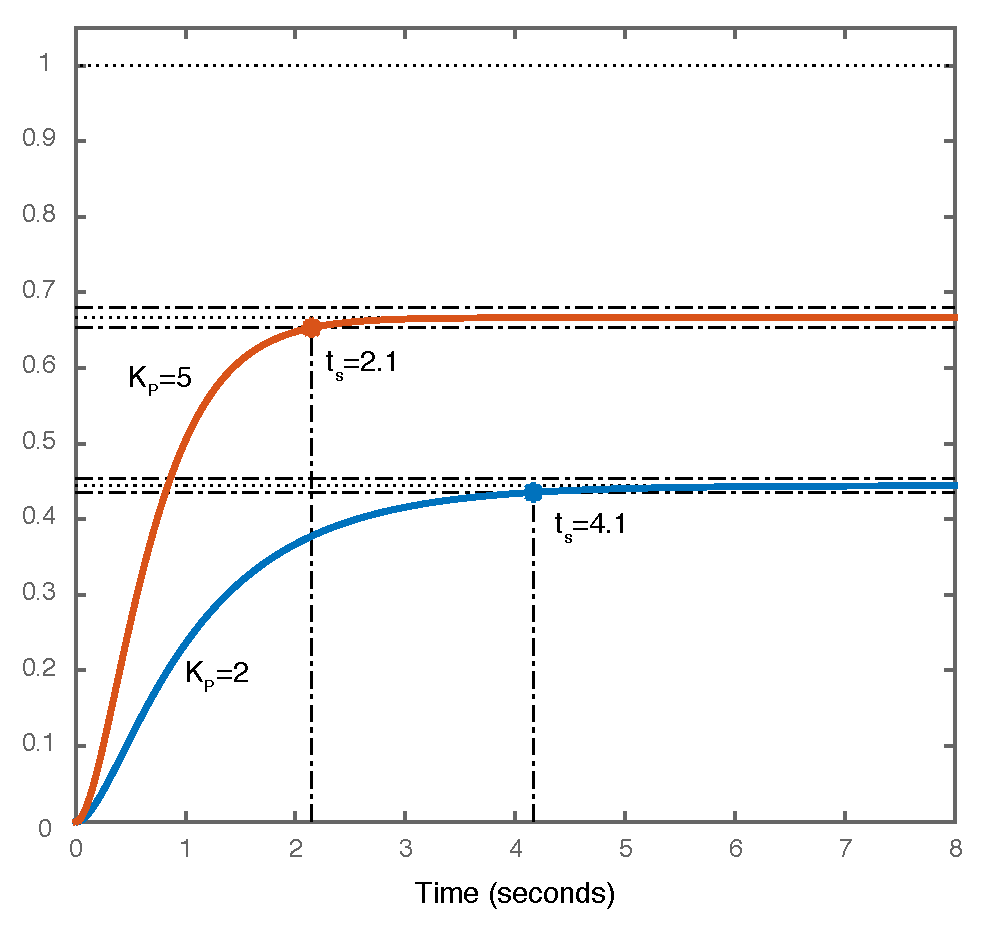
\includegraphics[width=0.4\textwidth]{Pcont1}
    \end{center}
  \end{minipage}

\vspace{12 pt}

We verify that both steady-state and transient performance increases
with larger $K_P$. However, we can also see that seetling time
estimation for $K_P = 5$ has a larger error, which expected
since the poles are close to each other thus violates the
dominant pole assumption. 


\textbf{Example 2:} Let $G(s) = \frac{1}{s^2 + 4 s + 5}$ (and under-damped
plant), then compute the unit-step steady state error for $K_p = 3$ and $K_P = 8$.
%
\begin{align*}
  e_{3} &= \frac{1}{1 + 3 / 5} \approx 0.625 \ , (\%62.5) 
\\
  e_{8} &= \frac{1}{1 + 8 / 5} \approx 0.385 \ , (\%38.5) 
\end{align*}
%
Obviously, stead-state performance is better with $K_p = 8$
compared to $K_p = 3$. Now compute the closed-loop poles
for $K_p = 3$ and $K_P = 8$, and estimate associated 
maximum overshoots
%
\begin{align*}
  T_3(s) = \frac{3}{s^2 + 4 s + 8} &\quad \rightarrow \
  p^{(3)}_{1,2} = -2 \pm 2 j  \quad M_P =M_P = e^{-pi / \tan \phi_3} =
                                     e^{-pi} \approx 0.04 \ (\%4)
\\
  T_8(s) = \frac{5}{s^2 + 4 s + 13} &\quad \rightarrow \
  p^{(8)}_{1,1} = -2 \pm 3 j  \quad M_P = e^{-pi / \tan \phi_8} =
                                      e^{-pi 2 / 3} \approx 0.12  \ (\%12)
\end{align*}
%
We can see that $K_P = 3$ provides a better transient performance
compared to $K_P = 8$, since both frequency oscillates and overs-shoot
is increased with a higher P gain. Now let's draw step-responses and
verify these observations. 

\vspace{12 pt}

  \begin{minipage}[h]{1\linewidth}
    \begin{center}
      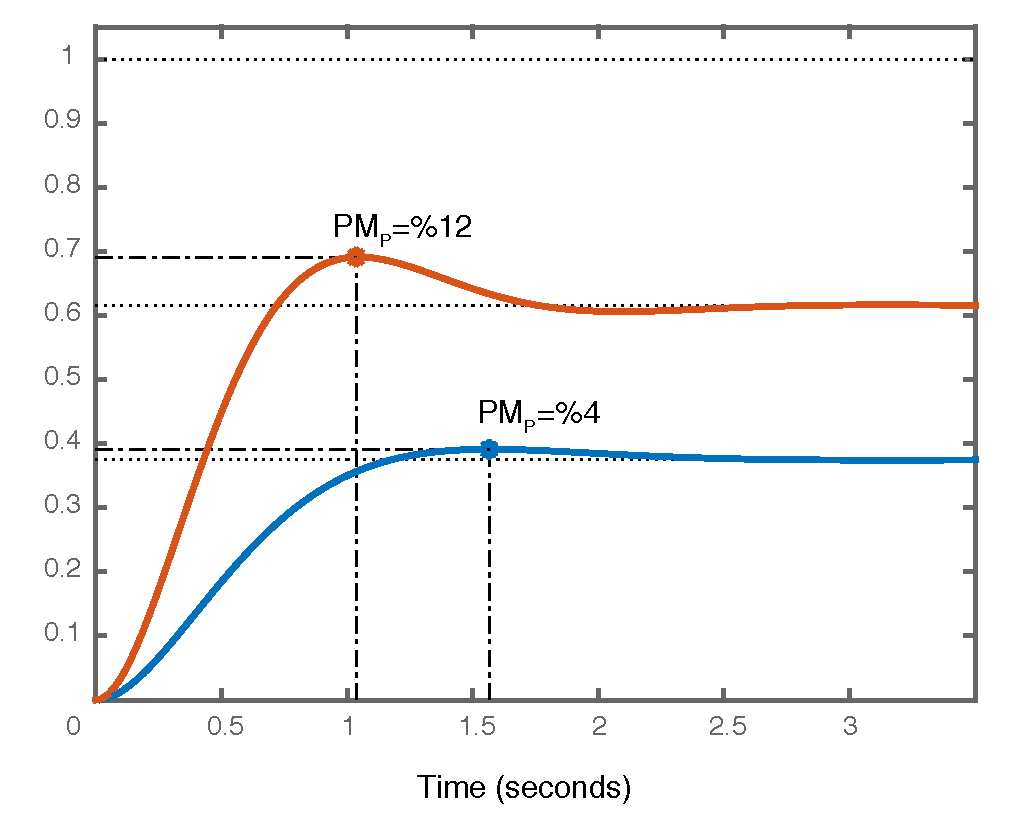
\includegraphics[width=0.4\textwidth]{Pcont2}
    \end{center}
  \end{minipage}

\vspace{12 pt}

We verify that stead-state performance is better with a larger
P gain. However, transent performance is worse with a
larger P-gain. This implies that if the plant is an under-damped
plant, then P controller has some serious limitations. 


\subsection{Proportional Derivative (PD) Controller}

In the classical form of PD controller, $C(s)$, takes the form
%
\begin{align*}
 C(s) = K_P + K_D s
\end{align*}
%
Let's first analyze the affect of $K_D$ term on steady-state 
performance on the same case ($2^{nd}$ order plant in standard form) 
%
\begin{align*}
  &G_{OL}(s) = \frac{K_P \omega_n^2 + K_D \omega_n^2 s}{s^2 + 2 \zeta
    \omega_n s + \omega_n^2}
\\
 Type \ 0 \quad K_p = K_P
\end{align*}
% 
Thus steady-state error for unit-step and unit-ramp inputs can be find
as
\begin{itemize}
\item Unit step: $e_{ss} = \frac{1}{1 + K_P}$, i.e. $K_p \nearrow \
  \Rightarrow \ e_{ss} \searrow$  
\\ Unit ramp: $e_{ss} = \infty$
\end{itemize}
  %
Obviously, $K_D$ has no effect on steady-state performance. Now
let's analyze the closed-loop transfer function
%
  \begin{align*}
  T(s) &= \frac{Y(s)}{R(s)} = \frac{K_P \omega_n^2 + K_D \omega_n^2 s}{s^2 + 2 \zeta
    \omega_n  s + \omega_n^2 + K_D \omega_n^2 s + K_P \omega_n^2}
\\
  &=   \frac{K_P \omega_n^2 + K_D \omega_n^2 s}{s^2 + ( 2 \zeta
    \omega_n + K_D \omega_n^2) s + (1 + K_P) \omega_n^2}
\\
,
\\
 \Bar{\omega}_n &= \sqrt{1 + K_P} \omega_n
\\
 \bar{\zeta} &= \frac{\zeta + K_D \omega_n / 2}{ \sqrt{ 1 + K_P} } 
  \end{align*}
%
We can see that
%
  \begin{align*}
    K_P \nearrow \ &\Rightarrow \ \omega_n \nearrow \ \& \ \zeta \searrow
\\
   K_D \nearrow \ &\Rightarrow \ \omega_n = \ \& \ \zeta \nearrow
  \end{align*}
%
In other words, for a second order system, we have full control on
closed-loop pole locations with PD control policy. Since, a high $K_P$
is required/preferred for steady-state performance (which couses 
the system to have overshoot and oscillatory behavior), $K_D$
term can be used to suppress oscillations and overshoot.
Note that in the closed-loop transfer function, numerator part
has a zero due to $K_D \omega_n^2 s$ term, which implies that
the closed-loop transfer function is not in standard $2^{nd}$ order
form. One should note the fact that, the existing of closed-loop
zero can affect the accuracy of our closed-loop transient performance
metric calculations (most probably deviations will be minor).
%

\textbf{Example 3:} Let $G(s) = \frac{1}{s^2 + 4 s + 5}$ (and under-damp
plant). Design a $PD$ controller such that steady-state error to
unit-step input is around $\% 20$ and the maximum percentage overshoot
is less than $\% 4$. 

\textbf{Solution:} We first design $K_D$ based on steady-state
requirement then choose $K_D$ based on the over-shoot requirement.
%
  \begin{align*}
    e_{ss} &= \frac{1}{1 + K_P/5} = 0.2
    \\
   K_P &= 20
  \end{align*} 
%
Now let's compte the closed-loop transfer function with $K_P = 20$.
  \begin{align*}
   T(s) &= \frac{20 + K_D s}{s^2 + (4 + K_D) s + 25}
  \end{align*} 
%
Let $K_D = 4$, than the closed-loop transfer function and associated
poles are computed as
%
  \begin{align*}
   T(s) &= \frac{20 + 4s}{s^2 + 8 s + 25}
  \\
  p_{1,2} = -4 \pm 3 j
  \end{align*} 
% 
We can estimate the overshoot based on the pole locations
%
  \begin{align*}
    PM_P = \% 100 e^{-\pi / \tan \phi} = e^{-\pi 4 / 3} = \% 1.5 < \% 4
  \end{align*} 
%
Let's plot the step-response of the resultant system and check if we
can meet the specifications.

\vspace{12 pt}

  \begin{minipage}[h]{1\linewidth}
    \begin{center}
      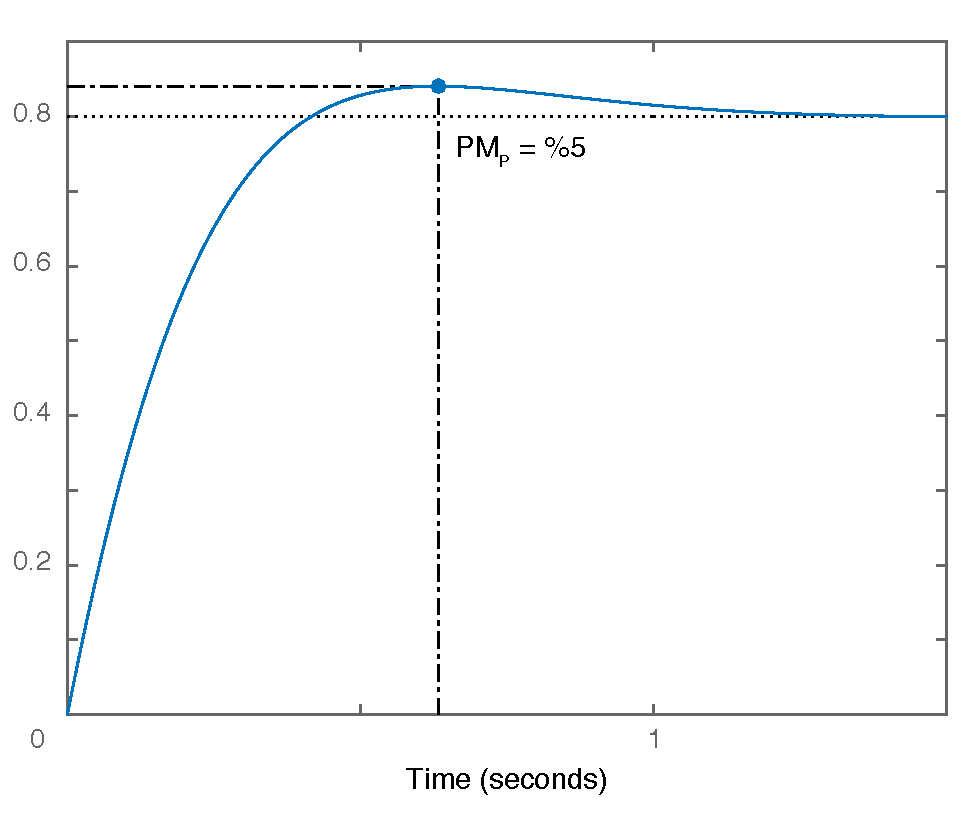
\includegraphics[width=0.4\textwidth]{PD1}
    \end{center}
  \end{minipage}

\vspace{12 pt}

We can observe that the computed over-shoot is $\% 5$, and indeed
higher than the requirement. Moreover, the gap between estimated
and numerically computed over-shoot is around $\%3.5$. Obviously,
the $K_D s = 4 s$ term in the numerator affects the output behavior and
its affect should be maximum when $0 < t < t_s$. In order see how
$K_D s = 4 s$, let's compre step responses of following transfer
functions
%
\begin{align*}
   T(s) &= \frac{20 + 4s}{s^2 + 8 s + 25}
  \\
   \hat{T}(s) &= \frac{20}{s^2 + 8 s + 25}
  \end{align*} 
% 
$T(s)$ and $\hat{T}(s)$ share the same poles and DC gain, but
$\hat{T}(s)$ is in standard form, thus has no zeros.

\vspace{12 pt}

  \begin{minipage}[h]{1\linewidth}
    \begin{center}
      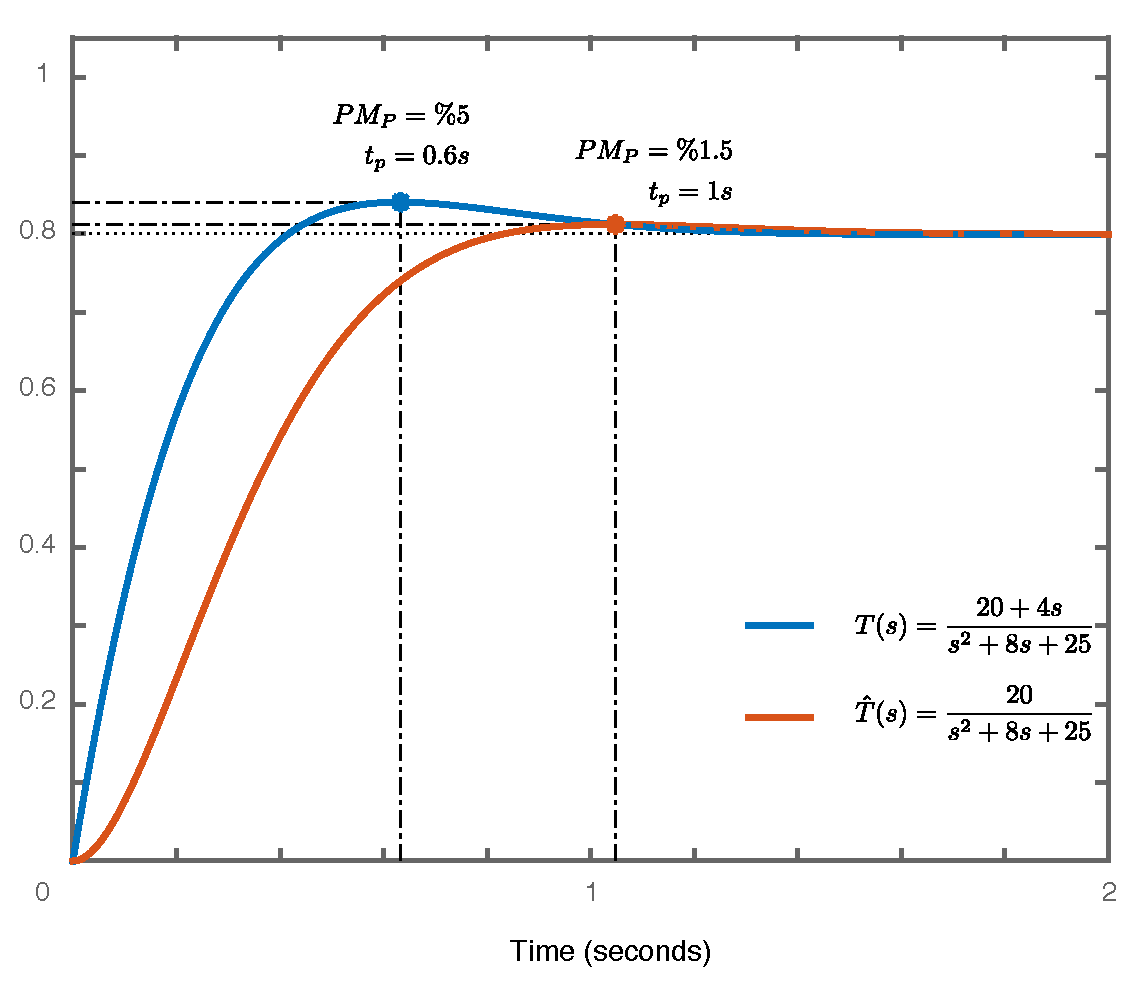
\includegraphics[width=0.4\textwidth]{zero}
    \end{center}
  \end{minipage}

\vspace{12 pt}

We can see that there exist non-negligible differences
between two transfer functions, which clearly shows that
the numerator dynamics can substantially affect the response.
In this context, we should think as the transient performance
metrics and associated approximate estimation formulas 
as heuristics which guides the design of controllers. 

\subsection{Integral (I) Controller}

Practical use of Integral controller (alone) is extremely 
rare, however we will analyze this case to better
understand the effect of Integral action on more useful
PI and PID topologies. 

In the pure Integral controller, $C(s)$, takes the form
%
\begin{align*}
 C(s) = K_I \frac{1}{s}
\end{align*}
%
Let's first analyze the steady-state 
performance where the plant is a $2^{nd}$ system in standard
%
\begin{align*}
  &G_{OL}(s) = \frac{K_I \omega_n^2}{s (s^2 + 2 \zeta
    \omega_n s + \omega_n^2)}
\\
 &Type \ 1 \quad K_v = K_I
\end{align*}
% 
Thus steady-state error for unit-step and unit-ramp inputs can be find
as
\begin{itemize}
\item Unit step: $e_{ss} = 0$ 
\item Unit ramp: $e_{ss} = \frac{1}{K_I}$, i.e. $K_I \nearrow \ \Rightarrow \ e_{ss} \searrow$  
\end{itemize}
  %
Basic idea is very clear, Integral action increases the type of the
system by introducing an extra pole at the origin (also increases the
total system order). Thus for a Type 0 plant, it completely eliminates 
the steady-state error for step-like inputs, and provides a
constant steady-state error for ramp-like inputs. 

Let's compte the closed-loop transfer function
%
\begin{align*}
T(s) = \frac{K_I \omega_n^2}{s^3 + 2 \zeta \omega_n s^2 + \omega_n^2 s
  + K_I \omega_n^2}
\end{align*}
  %
The closed loop system is now a third order system and
thus harder to analyze (we need new analysis tools). Moroever, 
we have only one paremeter $K_I$ and the closed-loop system has
three poles. One may easily guess that it is very hard to obtain 
a good performance with a pure Integral controller. 
Sometimes it bay be even quite hard to obtain a stable behavior.

\paragraph{Example 4:} Let's analyze the influence of an $I$ controller on a
first order plant in order to better understand the positive and
negative effects of $I$ action. Let $G(s) = \frac{1}{s+2}$.

The steady-state value of $y(t)$ (for unit-step input)
for the uncontrolled plant is $y_{ss} = 1/2$, thus we 
can say that steady-state error under unit-step input is 
$e_{ss} = 0.5$, where as for unit ramp it is easy to
show that $e_{ss} = \infty$. On the other hand, we can estimate the
settling time ($\%2$) for the uncontrolled plant as $t_{s} \approx 2.$

Now let's first analyze the setady-state performance under 
$C(s) = \frac{K_I}{s}$,
%
\begin{align*}
  &G_{OL}(s) = \frac{K_I }{s (s + 2)}
\\
 &Type \ 1 \quad K_v = K_I / 2
\end{align*}
% 
\begin{itemize}
\item Unit step: $e_{ss} = 0$ 
\item Unit ramp: $e_{ss} = \frac{2}{K_I}$, i.e. $K_I \nearrow \ \Rightarrow \ e_{ss} \searrow$  
\end{itemize}
 %
Obviously, steady-state performance improvement is 
significant (structurally). Now, lets
compute closed-lopp transfer function
%
\begin{align*}
  T(s) = \frac{K_I}{s^2 + 2 s + K_I}
\end{align*}
%
Now let's analyze the transient performance (settling time and maximum
overshoot) for $K_I = 1$ and $K_I = 2$ and compre them
w.r.t. uncontrolled plant
%
\begin{align*}
  K_I &= 1 \quad \rightarrow \quad \zeta = 1 \ , \ p_{1,2} = -1 \quad
        \rightarrow \quad M_P =0 \ , \ t_{s} \approx 4 s
\\
 K_I &= 2 \quad \rightarrow \quad \zeta = 1/\sqrt{2} \ , \ p_{1,2} =
       -1 + \pm j  \quad
        \rightarrow \quad M_P = 0.04 \ , \ t_{s} \approx 4 s
\end{align*}
% 
We can clearly see that integral action has a negative effect 
on transient performance. $K_I = 1$ case has a worse
settling time value than the original plant< 
Moroever we start to observe over-shoot at the output
when we increase integral gain to $K_I = 2$ case.

In order to illustrate these analytic observations, 
we plotted the step responses of original plant, 
closed-loop system with $K_I = 1$ and
closed-loop system with $K_I = 2$. 

\vspace{12 pt}

  \begin{minipage}[h]{1\linewidth}
    \begin{center}
      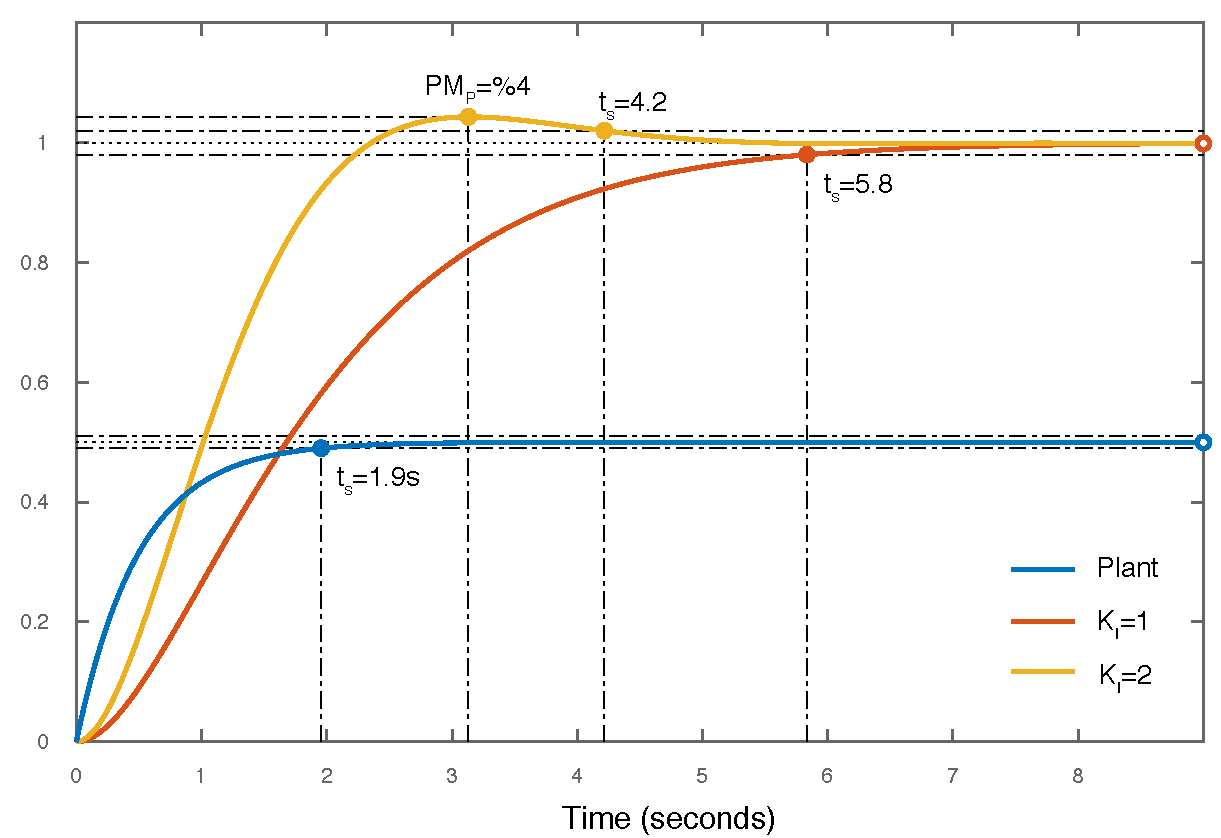
\includegraphics[width=0.7\textwidth]{PIcase}
    \end{center}
  \end{minipage}

\vspace{12 pt}

It is clear that PI controlle eliminates the
steady-state error, but we can also observe that
transient performance substantially degraded. In both cases
settling time is worse than the original plant,
and for case $K_I = 2$, overs-shoot is clear from the
figure. One interesting result is that settling time performance
for $K_I = 1$ (critically damped) is worse than $K_I = 2$
(under-damped) even though the approximate formula
provides the same estimate. The reason is that for the critically
damped case, the approximation under-estimates 
the settling time. 

In this context, we can conclude that
a little bit over-shoot could be good for the closed-loop
system from the perspective of settling time. 

\subsection{Proportional Integral (PI) Controller}

PI controller is commonly used in practical applications. 
In general, if a single P controller is satisfactory for 
transient requirements, but one seeks perfect steady-state
performance for unit-step like inputs, $PI$ is the first choice to
test (compared to PID). 

In the PI controller, $C(s)$, takes the form
%
\begin{align*}
 C(s) = K_P + \frac{K_I}{s}
\end{align*}
%
Let's first analyze the steady-state 
performance again with the plant is a $2^{nd}$ system in standard
%
\begin{align*}
  &G_{OL}(s) = \frac{K_P \omega_n^2 s +  K_I \omega_n^2}{s (s^2 + 2 \zeta
    \omega_n s + \omega_n^2)}
\\
 &Type \ 1 \quad K_v = K_I
\end{align*}
% 
Thus steady-state error for unit-step and unit-ramp inputs can be find
as
\begin{itemize}
\item Unit step: $e_{ss} = 0$ 
\item Unit ramp: $e_{ss} = \frac{1}{K_I}$, i.e. $K_I \nearrow \ \Rightarrow \ e_{ss} \searrow$  
\end{itemize}
  %
In other words $PI$ and $I$ controllers have same steady-state
performance characteristics. Now, let's compte the closed-loop transfer function
%
\begin{align*}
T(s) = \frac{K_P \omega_n^2 s + K_I \omega_n^2}{s^3 + 2 \zeta \omega_n
  s^2 + (1 + K_P) \omega_n^2 s
  + K_I \omega_n^2}
\end{align*}
  %
In this case, the closed-loop transfer function has three poles, 
and we have two parameters for tuning. Even though it provides a
much better framework than an I controller, still we need different tools
to tune the $K_I$ and $K_P$ gains.

\paragraph{Example 5:} Let's compre PI and I controllers using the
same plant in previous example, $G(s) = \frac{1}{s+2}$. We know that
PI controller has the transfer function form $C(s) = \frac{K_I}{s}$
and steady-state error characteristics can be derived as
%
\begin{align*}
  &G_{OL}(s) = \frac{s K_P + K_I }{s (s + 2)}
\\
 &Type \ 1 \quad K_v = K_I / 2
\\
&\mathrm{Unit} \ \mathrm{step :} \ e_{ss} = 0
\\
&\mathrm{Unit} \ \mathrm{ramp :} \ e_{ss} = e_{ss} = \frac{2}{K_I}
\end{align*}
% 
which are exactly same with the I controller. Now, lets
compute closed-lopp transfer function
%
\begin{align*}
  T(s) = \frac{K_D s + K_I}{s^2 + (2+K_D) s + K_I}
\end{align*}
%
Now let's choose $K_I = 8$ and $K_P = 4$, and estimate maximum
over-shoot and settling time for the closed-loop plant. 
%
\begin{align*}
p_{1} = -2 \ , \ p_{2} = -4
\quad \rightarrow \quad M_P = 0 \ , \ t_{s} \approx 2 s
\end{align*}
% 
These PI gains can match the settling time value
of the original plant without any over-shoot (since closed-loot
TF is over-damped).

Let's illustrate this analytic observations, by
plotting the step responses of the
closed-loop system with only integral controller with $K_I = 2$,
the closed-loop system with only integral controller with $K_I = 8$, 
and the closed-loop system with PI controller with $K_P = 4 \ , K_I = 8$. 

\vspace{12 pt}

  \begin{minipage}[h]{1\linewidth}
    \begin{center}
      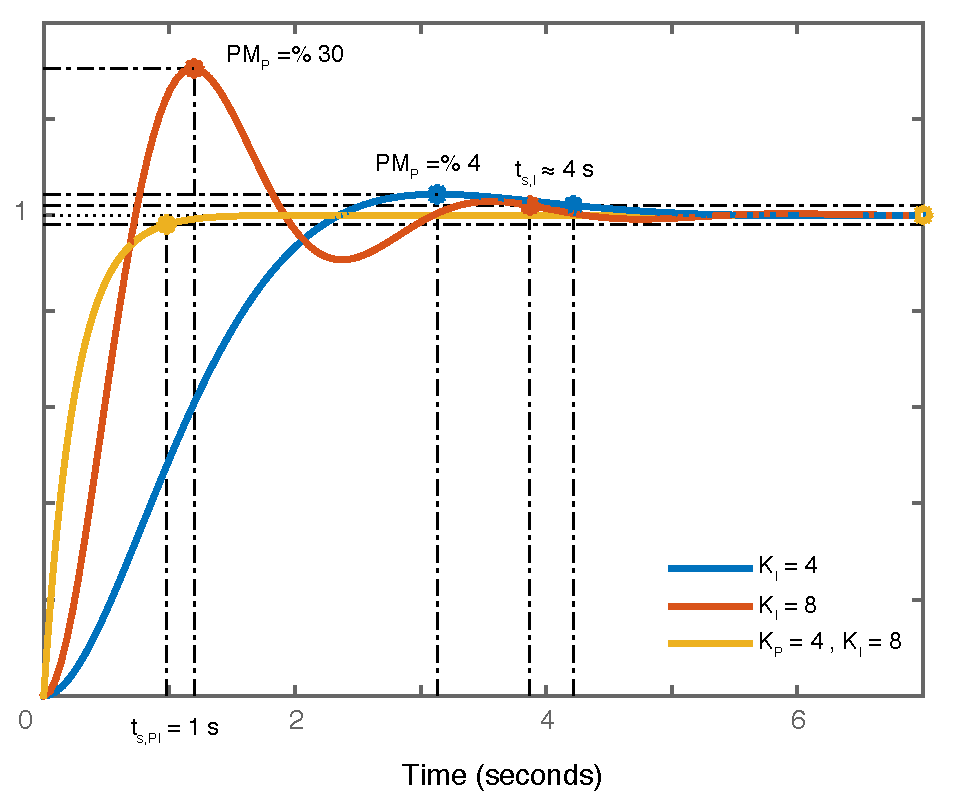
\includegraphics[width=0.65\textwidth]{IvsPI}
    \end{center}
  \end{minipage}

\vspace{12 pt}

In this illustration, we can see that settling time for both
I controllers is around $4 s$, however settling time for the
PI controller is $1 s$ which is even better than our estimation. 
The gap between settling time estimates come form the affect
of zero introduced by the PI controller. If one carefully, analyzes
the closed-loop transfer function he/she can see that a pole-zero
cancellation occurs (which may not be a good feature for practical
reasons). Technically, the closed-loop transfer function 
is reduced to a first order system in this case (????). 

We also see that when PI and I controllers has the same 
$K_I$ gain, the over-shoot in I controller is $\% 30$ which is very
high. 

\subsection{Proportional Integral Derivative (PID) Controller}

PID controller technically combines the advantages of 
the PD and PI controllers, with the trade of increased
parameter and implementation complexity. 
We know that PID controller has the following 
transfer function form
%
\begin{align*}
 C(s) = K_P + K_D s + \frac{K_I}{s}
\end{align*}
%
Let's first analyze the steady-state 
performance again where the plant is a $2^{nd}$ system in standard form
%
\begin{align*}
  &G_{OL}(s) = \frac{( K_D s^2 +  K_P s +  K_I ) \omega_n^2}{s (s^2 + 2 \zeta
    \omega_n s + \omega_n^2)}
\\
 &Type \ 1 \quad K_v = K_I
\end{align*}
% 
Thus steady-state error for unit-step and unit-ramp inputs can be find
as
\begin{itemize}
\item Unit step: $e_{ss} = 0$ 
\item Unit ramp: $e_{ss} = \frac{1}{K_I}$, i.e. $K_I \nearrow \ \Rightarrow \ e_{ss} \searrow$  
\end{itemize}
  %
In other words $PID$, $PI$, and $I$ controllers share the same steady-state
performance characteristics. Now, let's compte the closed-loop transfer function
%
\begin{align*}
  T(s) &= \frac{( K_D s^2 +  K_P s +  K_I ) \omega_n^2}{ s^3 + (2 \zeta
         \omega_n + K_D \omega_n^2) s^2 + (1 + K_P) \omega_n^2 s +  K_I}
\end{align*}
%
We can see that the closed-loop transfer function has three poles, and
we have three parameters to tune. If we have no limits on gains, we
can place the closed-loop poles to any desired location. However,
numerator has now two zeros, thus it is now harder to predict the
affect of closed-loop zeros on the output behavior. 

\textbf{Example 4:} Let $G(s) = \frac{1}{s^2 + 4 s + 5}$, Design a
PID controller such that we observe zero unit-step steady state error, 
maximum percent overs-shoot is less than $\% 5$, and settling time 
is around $1 s$. 

\textbf{Solution:} We already know that PID controller for a Type 0
plant completely eliminates the unit-step steady state error. Now 
let's compte closed-loop transfer function
%
\begin{align*}
  T(s) &= \frac{K_D s^2 +  K_P s +  K_I}{ s^3 + (4 + K_D) s^2 + (5 +K_P) s +  K_I}
\end{align*}
%
One way of choosing appropriate pole locations for a third-order
closed-loop system is placing one of the poles (a real one) far away from the
other poles such that closed-loop system shows a second order
like behavior. We require that maximum over shoot of $\% 5$
and settling time is around $1 s$. Let the dominant poles of the
closed-loop system be
%
\begin{align*}
  p_{1,2} = -4 \pm 3 j
\end{align*}
%
Settling time and maximum overs-shoot associated with this
closed-loop poles can be estimated as
%
\begin{align*}
 t_s \approx 1 s
\\
M_P \approx e^{-pi 4/3} = 0.015 
\end{align*}
%
These estimates satisfy the requirements. Let $p_3 = 3 (-4) = -12$, then
desired characteristic equation takes the form
%
\begin{align*}
d^*(s) = (s + 12)(s^2 + 8 s + 25) = s^2 + 20 s + 121 s + 300
\end{align*}
% 
Then, we can compute the PID gains as
%
\begin{align*}
  K_P &=  116 \\
  K_I &= 300 \\
  K_D &= 16\\
\end{align*}
%
The first thing, we can observe is that the quantitive values of the gains 
seem to be much larger than the gains that we played before.
In general, if we want to improve the performance of both
steady-state and transient characteristics by implementing PID 
topology instead of P, PI, or PD the gain values would go up
which may cause practical problems and potentially
can be costly in terms of energetic performance. 

Now let's plot the step response of the closed-loop
system and try to verify these analytic observations

\vspace{12 pt}

  \begin{minipage}[h]{1\linewidth}
    \begin{center}
      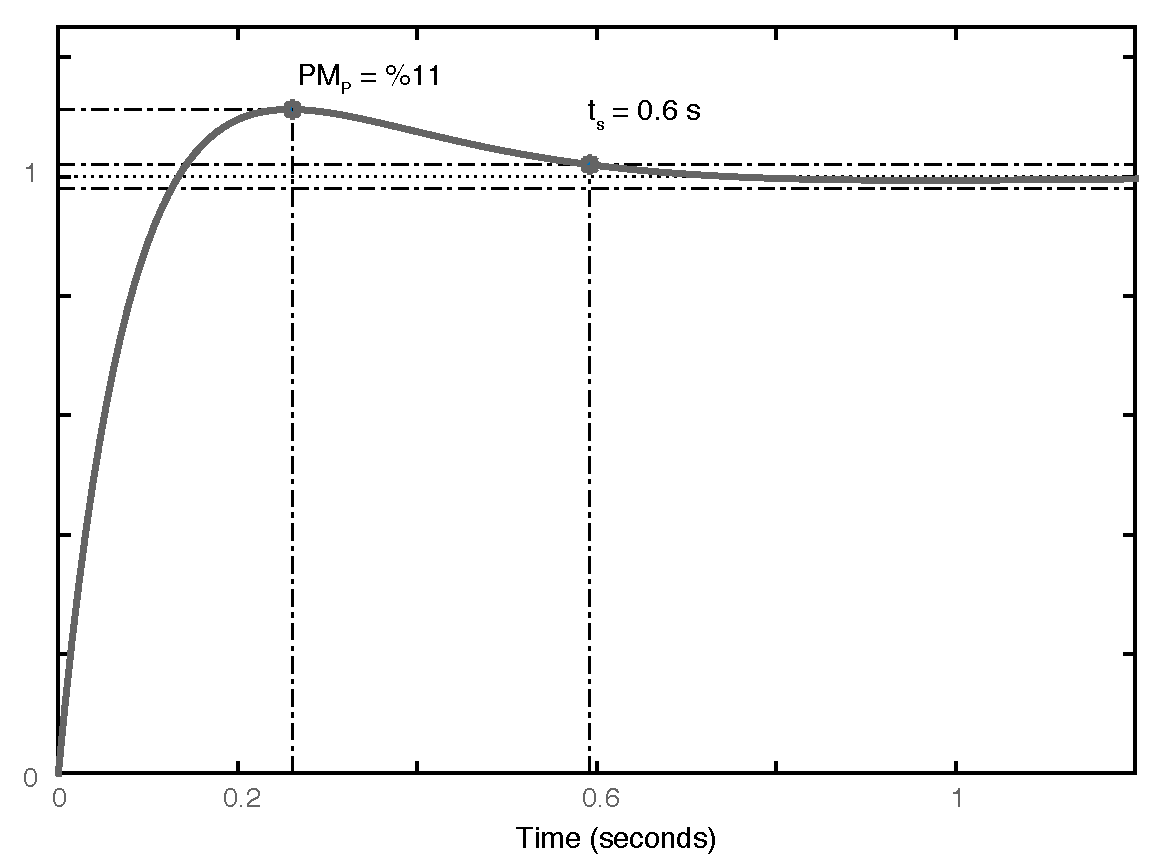
\includegraphics[width=0.5\textwidth]{PIDe}
    \end{center}
  \end{minipage}

\vspace{12 pt}

We can see that the settling time in numerical simulation
is much better than our estimate $0.6 s < 1 s$, however
numerical percentage over-shoot is higher than our estimate, 
$\% 11 > \% 1.5$, and does not meet our specifications. 
The core reason behind this is that it is basically harder to
tune a PID controller compared to P, PD, and PI controllers
due to increased parametric complexity and (may be more importantly)
$2^{nd}$ numerator dynamics introduced with the PID control 
policy.




% **** This ENDS THE EXAMPLES. DON'T DELETE THE FOLLOWING LINE:
\end{document}